\documentclass{article}

\usepackage[utf8]{inputenc}
\usepackage[]{amsmath}
\usepackage[english]{babel}
\usepackage[]{amsthm} %lets us use \begin{proof}
\usepackage[]{amssymb} %gives us the character \varnothing
\usepackage{graphicx}
\usepackage{float}
\DeclareMathOperator*{\argmin}{argmin}
\DeclareMathOperator*{\argmax}{argmax}

\title{Optimal k-means vs. Bayes Decision Rule}
\author{Thomas Athey}
\date\today

\begin{document}
\maketitle
\section{Problem Definition}

%********************************
\subsection{K Means}
Say we have the dataset \[ X=\{x_1,x_2,\ldots,x_n\} \: \epsilon \: (R^p)^n \] that we seek to partition into $k$ clusters. The k-means algorithm seeks to find the cluster centers:\\
\[C=\{c_1,c_2,\ldots,c_k\} \: \epsilon \: (R^p)^k\]
and the cluster assignments 
\[ A = \{ a_1,a_2,\ldots,a_n\} \: \epsilon \: \{1,2,\ldots,k\}^n \]
that minimize the cost function:
\[ J = \frac{1}{n} \sum\limits_{i=1}^n ||x_i - c_{a_i} ||_2^2\]

%********************************
\subsection {K Means Decision Rule}
Given a set of centers $C$, it is obvious that the optimal decision rule ($D:R^p \to {1,2,\ldots,k}$) assigns each point $x_i$ to the closest centers i.e.
\begin{equation}
\label{eq:a}
D(x_i) = a_i =\argmin_j   ||x_i - c_{j} ||_2^2
\end{equation}
\quad This process of assigning datapoints to clusters can be thought of as a decision rule. This decision rule will involve linear boundaries between clusters since the relative proximity of two different cluster centers only changes along the axis that spans the two centers. Now, let's flip this problem around. Given a descision rule comprised of a set of linear decision boundaries ($D$), the ideal cluster centers are, obviously, the means of each cluster i.e.
\[ c_j = \frac{ \sum\limits_{i=1}^n x_i*I(a_i == j)} {\sum\limits_{i=1}^n I(a_i == j)} \]
where $I(x)$ is the indicator function of the boolean x. \\
\null \quad Say that each $X_i$ is an iid random variable that follows some distribution $f_X$. Given some decision rule with linear boundaries ($D$), and thus a set of cluster centers ($C_D$), the cluster assignment, $D(X)$ is a random variable according to \ref{eq:a}. \\ \null \quad
The law of large numbers tells us that:
\begin{equation}
\label{eq:JD}
 J_D = \lim_{n\to\infty} J = E[||X - c_{D(X)}||_2^2] = E_{D(X)}[E_{X|D(X)=a}[||X - c_a||_2^2]]
\end{equation}
Finally, let us define the optimal large sample k-means decision rule, $D_k^*$, as:
\begin{equation}
\label{eq:Dk*}
D_k^*(x) = \argmin_D J_D 
\end{equation}
where $J_D$ is defined in \ref{eq:JD}.


%********************************
\subsection {Bayes Decision Rule of Mixture Distribution}
\quad We are studying clustering in the context of underlying mixture distributions. A typical form of a mixture distribution is a weighted sum of the same parameterized distribution, with each component having its own set of parameters. A k-mixture of a distribution f is defined as:
\begin{equation}
\label{eq:mix}
f_X(x) = \sum\limits_{i=1}^k \tau_i * f(x;\theta_i)
\end{equation}
where $f$ may be, for example, the normal distribution, in which case $\theta_i = \{\mu_i,\Sigma_i\}$. \\
\null \quad This distribution can be interpreted as the distribution of X marginalized over the hidden cluster assignment A i.e.:
\[
Pr(A=a) = \tau_a
\]
\[
f_{X|A=a}(x) = f(x;\theta_a)
\]
\null \quad The Bayes decision rule, $D_B^*$ chooses the value of A that minimizes the probability of error i.e.:
\[ D_B^*(x) = \argmin_a Pr(A \neq a | X=x) \]

\subsection{Problem}
\null \quad We want to characterize the settings where $D_k^* = D_B^*$.



\section{MGFs}
\subsection{MGF of Mixture}
\quad The moment generation function (MGF) of a random variable, $X$, is defined as:
\[ M_X(t) = E_X[e^{t^Tx}]\]
\quad Due to linearity of expectation, the MGF of the mixture distribution is the weighted sum of the MGFs of the components. Say X is distributed according to \ref{eq:mix}, and the MGF associated with $f(x;\theta_i)$ is $M_i$, then:
\begin{equation}
\label{eq:mgfmix}
M_X(t) = \sum\limits_{i=1}^k \tau_i * M_i(t)
\end{equation}

\subsection{MGF of a Normal Mixture split in Half}
\quad In k-means, we partition the space of $R^p$ into halfspaces and calculate the first two moments of $X$ within these partitions. We calculate first moments to get cluster centers $C$, and second moments to get costs $J$. Here we present a series of equations that can be assmebled to find an explicit expression of the MGF of "half of a mixture" i.e. $I(u^Tx > c)*f_X$.
\begin{equation}
\label{eq:q}
q_i = \int_{u^Tx = c}^{\infty} N(x;\mu_i,\Sigma_i)dx = \frac{1}{2}erfc(\frac{c - u^T\mu_i}{||D_i^{1/2}U_i^Tu||\sqrt{2}})
\end{equation}
where $erfc(x)$ is the complementary error function and $\Sigma_i = U_iD_iU_i^T $ is the diagonalization of $\Sigma$.

\begin{equation}
\label{eq:m}
m_i(t) = \int_{u^Tx=c}^{\infty} e^{t^Tx}N(x;\mu_i,\Sigma_i)dx = \frac{1}{2}e^{\mu_i^Tt + \frac{1}{2}t^T\Sigma_i t}erfc(\frac{c-u^T(\mu_i+\Sigma_i t)}{||D_i^{1/2}U_i^Tu||\sqrt{2}})
\end{equation}

\quad The derivation of both \ref{eq:q} and \ref{eq:m} involve the substitution $y=Ux$ where $U$ is a unitary matrix whose first row is the $u^T/||u||$. \ref{eq:m} also uses completing the square within the exponent. \\

\begin{equation}
\label{eq:mgf}
M_{X|u^TX>c}(t) = \frac{\sum\limits_{i=1}^k \tau_i m_i(t)}{\sum\limits_{i=1}^k \tau_i q_i}
\end{equation}
where X is in the halfspace $u^TX > c$. \\
\null \quad Now we can take derivatives of the MGF to get moments, here we find the first two moments. With $s_i=\mu_i^Tt+\frac{1}{2}t^T\Sigma_i t$ and $z_i(t) = \frac{c - u^T(\mu_i + \Sigma_i t)}{||D_i^{1/2}U_i^Tu||\sqrt{2}}$:
\begin{equation}
\triangledown_tm_i(t) = \frac{1}{2}e^{s_i}(erfc(z_i)(\mu_i+\Sigma_i t) + \sqrt{\frac{2}{\pi}}e^{-z_i^2}\frac{\Sigma_i u}{||D_i^{1/2}U_i^Tu||})
\end{equation}
\begin{equation}
\triangledown_tm_i(t) |_{t=0}= \frac{1}{2}(erfc(z_i(0))\mu_i + \sqrt{\frac{2}{\pi}}e^{-z_i(0)^2}\frac{\Sigma_i u}{||D_i^{1/2}U_i^Tu||})
\end{equation}
And,
\begin{equation}
E[X|u^TX>c] =  \frac{\sum\limits_{i=1}^k \tau_i \triangledown_t m_i(t)}{\sum\limits_{i=1}^k \tau_i q_i}
\end{equation}
And the second moment is:
\begin{equation}
\begin{split}
H_t(m_i(t)) = \frac{1}{2}e^{s_i}[erfc(z_i)((\mu_i + \Sigma_it)(\mu_i + \Sigma_it)^T + \Sigma_i) + \\ \sqrt{\frac{2}{\pi}}\frac{e^{-z_i^2}}{||D_i^{1/2}U_i^Tu||} (\Sigma_i u (\mu_i + \Sigma_i t)^T + (\mu_i + \Sigma_i t)(\Sigma_i u)^T +  \frac{z_i  \sqrt{2}}{||D_i^{1/2}U_i^Tu||}\Sigma_i u u^T \Sigma_i)]
\end{split}
\end{equation}

\begin{equation}
\begin{split}
H_t(m_i(t))|_{t=0} = \frac{1}{2}[erfc(z_i(0))(\mu_i\mu_i^T + \Sigma_i) + \\ \sqrt{\frac{2}{\pi}}\frac{e^{-z_i(0)^2}}{||D_i^{1/2}U_i^Tu||} (\Sigma_i u \mu_i^T + \mu_i u^T \Sigma_i + \frac{z_i(0) \sqrt{2}}{||D_i^{1/2}U_i^Tu||}\Sigma_i u u^T \Sigma_i)]
\end{split}
\end{equation}

And,
\begin{equation}
Var[X|u^TX>c] =  \frac{\sum\limits_{i=1}^k \tau_i H_t(m_i(t))}{\sum\limits_{i=1}^k \tau_i q_i} - E[X|u^TX>c] (E[X|u^TX>c])^T
\end{equation}

The previous results applied to the half space defined by $u^TX > c$, finding the results for the other half space is easy, recall that $m_i$ and $q_i$ are integrals over a half space: 
\begin{equation}
g(t;u,c) = \int_{u^Tx=c}^\infty f(x,t)dx
\end{equation}
Let's look at the same integral over the other half space:
\begin{equation}
 \int_{-\infty}^{u^Tx=c} f(x,t)dx =  \int_{-u^Tx=-c}^\infty f(x,t)dx=g(t;-u,-c)
\end{equation}
\quad Thus, we can find the MGF of the other half space by plugging in -u and -c. Further, we take derivatives with respect to t to find moments so, again, plugging in -u and -c will give the complementary moments. We denote these complementary values with a prime (') i.e. since $q_i=Pr(u^TX>c)$, we say $q_i'=Pr(u^TX<c)$\\

\quad Lastly, note that in the k-means framework, the expected loss given that the decision boundary is defined by $u$ and $c$ is:
\begin{equation}
E[J|u,c] = (\sum\limits_{i=1}^k \tau_i q_i)*tr(Var[X|u^TX>c]) + (\sum\limits_{i=1}^k \tau_i q_i')*tr(Var[X|u^TX<c])
\end{equation}

\section{Simplest Case}
Let us try to solve our initial problem ($D_k^* = D_B^*$) where we are in 1-D, and k=2 with $\tau_1=\tau_2=1/2$, $\mu_1 = -m$, $\mu_2 = m$, and $\Sigma_1 = \Sigma_2 = 1$ and our decision boundary is at c. In this case:
\subsection{Region $X > c$} 
\[ z_1 = \frac{c+m}{\sqrt{2}} \]
\[ z_2 = \frac{c-m}{\sqrt{2}} \]
\[ q_1 = \frac{1}{2} erfc(z_1)\]
\[ q_2 = \frac{1}{2} erfc(z_2)\]
\[ \triangledown_t m_1|_{t=0} = \frac{1}{2}(-erfc(z_1)*m +\sqrt{\frac{2}{\pi}} e^{-z_1^2}) \]
\[ \triangledown_t m_2|_{t=0} = \frac{1}{2}(erfc(z_2)*m +\sqrt{\frac{2}{\pi}} e^{-z_2^2}) \]
\[ E[X|X>c]= \frac{m*(erfc(z_2) - erfc(z_1)) + \sqrt{\frac{2}{\pi}}*(e^{-z_1^2}+e^{-z_2^2})}{2(q_1+q_2)}\] 
\[ H_t(m_1(t))|_{t=0} = \frac{1}{2}[erfc(z_1)(m^2+1)+\sqrt{\frac{2}{\pi}}e^{-z_1^2}(-2m+z_1 \sqrt{2})]\]
\[ H_t(m_2(t))|_{t=0} = \frac{1}{2}[erfc(z_2)(m^2+1)+\sqrt{\frac{2}{\pi}}e^{-z_2^2}(2m+z_2 \sqrt{2})]\]

\[ Var(X|X>0) =  \frac{ H_t(m_1(t))|_{t=0} +  H_t(m_2(t))|_{t=0}}{q_1+q_2} -
E[X|X>c]^2 \]

\subsection{Region $X < c$}
All we need to do is define
\[ z_1' = \frac{-c+m}{\sqrt{2}} = -z_2\]
\[ z_2' = \frac{-c-m}{\sqrt{2}} = -z_1\]
Then the rest of the equations are identical to those in section 3.1 after we replace $z_1$ with $z_1'$ and $z_2$ with $z_2'$.

\subsection{K-means Cost}
Here we use equation \ref{eq:JD} with the decision rule:
 \[ 
D(x) =
  \begin{cases} 
      1 & x < c \\
      2 &  x\geq c \\
   \end{cases}
\]
\begin{equation}
\begin{split}
J_D = Pr(X<c) * Var(X|X<c) + Pr(X>c)*Var(X|X>c) = \\
\frac{1}{2}(q_1' + q_2') Var(X|X<c) + \frac{1}{2}(q_1 + q_2) Var(X|X>c) = \\
m^2 + 1 - \frac{1}{2}((q_1'+q_2')E[X|X<c]^2 + (q_1+q_2)E[X|X>c]^2)
\end{split}
\end{equation}


So, we seek, 
\[ c^* = \argmin_c J_D \]
We should expect (and surely hope) that $c^* = 0$, the Bayes optimal decision rule. Below is a graph of the cost function at varying c, giving evidence that the optimal k means rule indeed recovers the Bayes optimal rule.


\begin{figure}[H]
\begin{center}
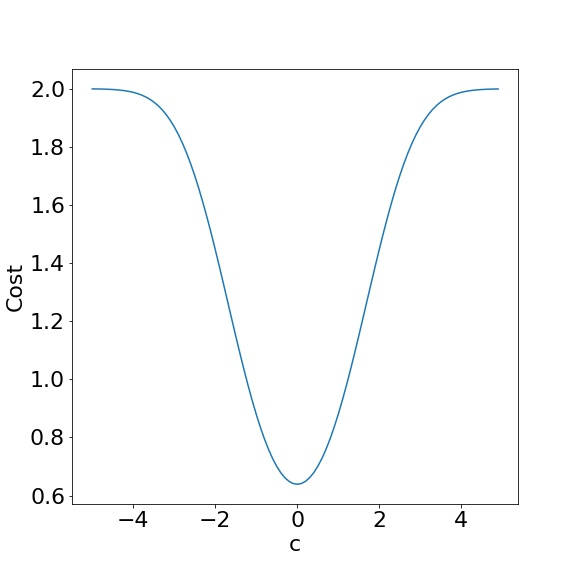
\includegraphics[scale=0.24]{simple_cost.jpg}
\end{center}
\caption{Simple Case with m=1: Cost function at different decision rules.}
\label{fig:simple_cost}
\end{figure}

Returning to the cost function:
\[ c^* = \argmin_c J_D = \argmax_c \; (q_1'+q_2')E[X|X<c]^2 + (q_1+q_2)E[X|X>c]^2\]
This is a sum of two terms that each depend on c. When we revisit the equations from Section 3.1, we notice the two terms are identical, except for the sign change in c. 
\[ f(c) = (q_1'+q_2')E[X|X<c]^2 \Rightarrow f(-c) =  (q_1+q_2)E[X|X>c]^2\]
i.e.
\[ c^* = \argmax_c f(c) + f(-c)\]
where $f(c)$ is a differentiable function. Clearly, $f(c) + f(-c)$ has a local extremum at $c=0$, so we just need to consider whether this local extremum is a global extremum.




\end{document}